\begin{comment}
- Gibs phenomenon
- Post-processing used (how impactful is removing non-distinct solutions?)
- How does clean TVD evolve with JVV steps (see proof)?
- Approximation ratio
- Numerical analysis (which mean to take)
\end{comment}

\chapter{Résolution de problèmes \textsf{\#P}-complet avec VQCount}

%-----------------------------------------------------------------------------%

\begin{comment}
\subsection*{Plan}

\begin{enumerate}
    \item Mentionner les problèmes étudiés
    \item Mentionner les méthodes utilisées (réseaux de tenseurs)
    \item Décrire les paramètres de l'étude (nombre d'instances, régimes de complexité, etc.)
    \item Expliquer les principaux résultats (compromis entre QAOA et GM-QAOA)
\end{enumerate}

\subsection*{Références}
\end{comment}

Dans la section précédente, un cadre théorique s'appuyant sur l'algorithme de JVV a été construit pour la résolution de problèmes de comptage à l'aide d'algorithmes variationnels quantiques. L'algorithme résultant, VQCount, obtient un compte approximatif à une erreur multiplicative près en échantillonnant un nombre polynomial de solutions à un circuit quantique optimisé GM-QAOA. Toutefois, plusieurs conditions potentiellement dispensables ou difficilement applicables ont été imposées. Cette section change l'optique précédente en évaluant l'algorithme VQCount uniquement en tant que méthode heuristique, c'est-à-dire en caractérisant l'algorithme sans se soucier des garanties. la résolution de deux problèmes \textsf{\#P}-complet, \#NAE3SAT et \#1in3SAT, sont étudiés.

%-----------------------------------------------------------------------------%

\section{Paramètres de l'étude}


Certaines précédentes considérations sont ainsi relâchées ou modifiées. D'abord, l'algorithme GM-QAOA n'est plus considéré dans sa forme limite de Grover. Les paramètres $(\vec{\alpha}, \vec{\beta})$ sont optimisées plutôt que d'utiliser des paramètres fixes. De plus, les problèmes étudiés sont transformé à des Hamiltonians de problème régulier contenant une tour d'états excités plutôt que de l'oracle à deux niveaux construits précédemment.

L'algorithme VQCount est appliqué aux problèmes \#NAE3SAT positif et \#1-in-3SAT positif présentés à la section~\ref{sec:satisfaisabilite-booleenne}. Le problème \#NAE3SAT est difficile près du seuil de satisfaisabilité situé au ratio de clauses sur variables critique $\alpha_{c} \approx 2.1$. Pour étudier l'effet de la complexité des formules aléatoires sur la performance de VQCount, des instances sont générées à $\alpha = 1$ et $\alpha = 2$. Celles-ci sont générées à partir de graphes connectés biparties, imposant une restriction supplémentaire. Similairement, les instances du problème \#1-in-3SAT positive sont à leur seuil de difficulté le plus élevé près de $\alpha_{c} \approx 2/3$. Pour étudier ce problème dans le régime difficile, les instances sont générées à partir de graphes aléatoires cubiques, en plaçant une clause sur tous les sommets et une variable sur toutes les arrêtes. Ce type de problème appartient à la catégorie des problèmes verrouillés, décrit à la section~\ref{sec:transitions-de-phase}, étant vraisemblablement les plus plus difficiles des problèmes \#P. Par la suite, les instances générées sont convertis en un modèle d'Ising à l'aide de la transformation décrite à la section~\ref{subsec:encodage-probleme}.

La simulation de circuits quantiques est un problème complexe en raison de la quantité de mémoire nécessaire pour représenter l'espace d'Hilbert. La méthode la plus utilisée, la simulation à vecteur d'état, ne peut atteindre plus d'une vingtaine de qubits pour cette raison. Les réseaux de tenseur sont un outil alternatif puissant, particulièrement pour l'étude de circuits quantiques peu profonds. L'annexe~\ref{cha:reseaux-de-tenseurs} introduit les réseaux de tenseur et les méthodes particulières utilisées pour la simulation de l'algorithme VQCount. La librairie « Quimb »~\cite{grayQuimbPythonPackage2018} est utilisé pour modéliser l'optimisation et l'échantillonnage des circuits quantiques QAOA et GM-QAOA. Les paramètres de ces circuits sont optimisés avec la programmation séquentielle des moindres carrés tel qu'implémenté par la librairie « SciPy »~\cite{virtanenSciPy10Fundamental2020}. Pour évaluer la validité des résultats obtenus, « Ganak »~\cite{sharmaGANAKScalableProbabilistic2019}, un compteur de modèles exact basé sur une approche probabiliste, est utilisé pour trouver le nombre exact de solutions et le solveur SAT « Glucose3 »~\cite{eenExtensibleSATsolver2004,audemardPredictingLearntClauses2009} , implémenté dans l'ensemble d'outils « PySAT »~\cite{ignatievPySATPythonToolkit2018}, est utilisé pour énumérer toutes les solutions.

Pour le problème \#NAE3SAT, 20 instances aléatoires sont générées par taille d'instance, allant de 6 à 20 variables, pour les deux densités de clause $\alpha=1$ et $\alpha = 2$. Similairement, problème \#1-in-3SAT, 20 instances aléatoires sont générées pour une taille de variable allant de 9 à 27 variables par saut de 3 variables, pour une densité de clause $\alpha = 2/3$. 


%-----------------------------------------------------------------------------%

\section{Biais d'échantillonage}

\begin{comment}
\subsection*{Plan}

\begin{enumerate}
    \item Décrire le comportement de la non-uniformité pour les différents problèmes (ne pas oublier 2SAT)
\end{enumerate}
\end{comment}




\begin{figure}[h]
    \centering
    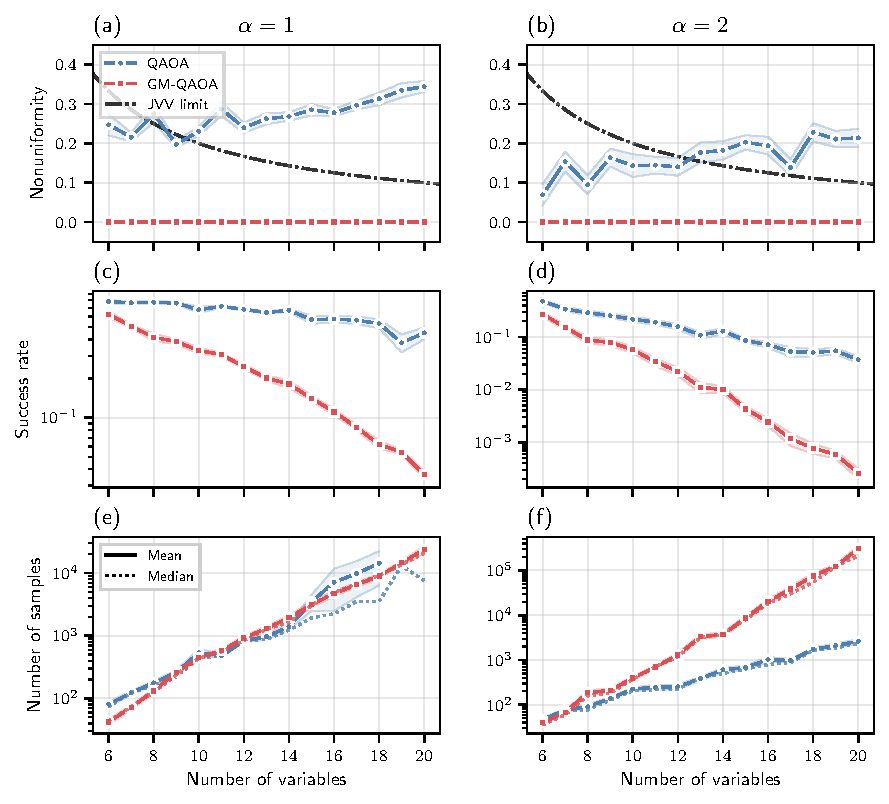
\includegraphics[width=1\textwidth]{figures/nae3sat-number-of-samples.pdf}
    \caption{}
    \label{fig:nae3sat-number-of-samples}
\end{figure}

\begin{figure}[h]
    \centering
    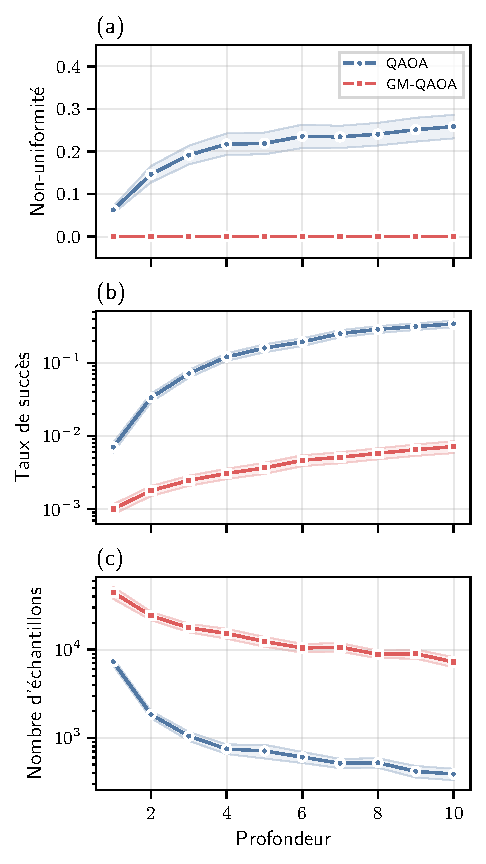
\includegraphics[width=0.5\textwidth]{figures/nae3sat-depth.pdf}
    \caption{}
    \label{fig:nae3sat-depth}
\end{figure}

\begin{figure}[h]
    \centering
    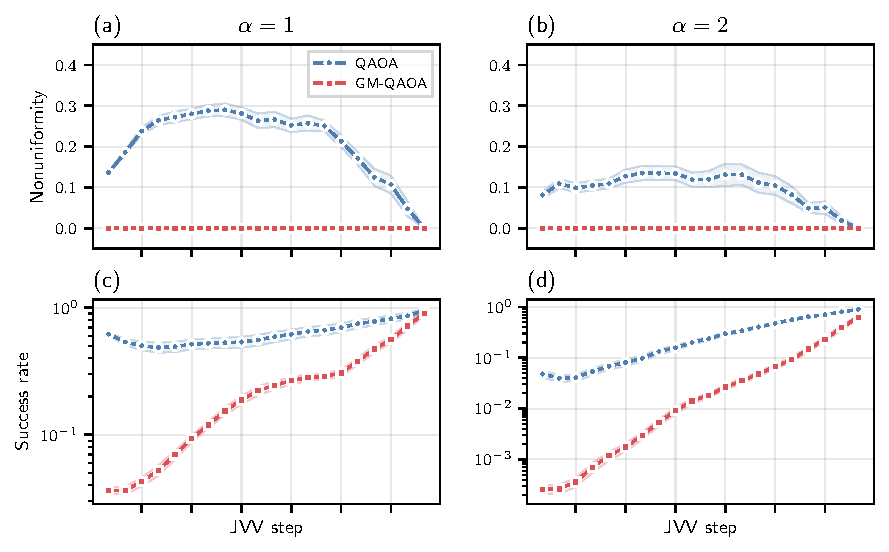
\includegraphics[width=1\textwidth]{figures/nae3sat-jvv-steps}
    \caption{}
    \label{fig:nae3sat-jvv-steps}
\end{figure}

%-----------------------------------------------------------------------------%


\section{Performance}

\subsection*{Plan}

\begin{enumerate}
    \item  Décrire le taux de réussite et le nombre d'échantillons requis
    \item  Décrire la performance de l'algorithme en fonction de la profondeur du circuit
    \item Décrire l'efficacité d'échantillonage et la précision du compte
    \item Présenter brièvement le ratio d'approximation
\end{enumerate}

\subsection*{Références}

%-----------------------------------------------------------------------------%
